% Chapter 1

\chapter{Introducción general} % Main chapter title

\label{Chapter1} % For referencing the chapter elsewhere, use \ref{Chapter1} 
\label{IntroGeneral}

En el presente capítulo se introduce el área en la que se enmarca el trabajo, se describe el contexto y la motivación que dieron origen al desarrollo, se revisan las soluciones existentes para problemas similares y se enuncian los objetivos perseguidos. El problema abordado es la gestión manual de los pedidos que los comercios reciben por canales de mensajería, y su resolución resulta relevante por el volumen de operaciones que hoy se procesan de esa forma.

%----------------------------------------------------------------------------------------

% Define some commands to keep the formatting separated from the content 
\newcommand{\keyword}[1]{\textbf{#1}}
\newcommand{\tabhead}[1]{\textbf{#1}}
\newcommand{\code}[1]{\texttt{#1}}
\newcommand{\file}[1]{\texttt{\bfseries#1}}
\newcommand{\option}[1]{\texttt{\itshape#1}}
\newcommand{\grados}{$^{\circ}$}

%----------------------------------------------------------------------------------------

%\section{Introducción}

%----------------------------------------------------------------------------------------



%----------------------------------------------------------------------------------------
%	SECTION 1
%----------------------------------------------------------------------------------------
 
\section{Mensajería instantánea y gestión de pedidos en comercios minoristas}
\label{sec:intro_general}
 
La creciente adopción de canales de mensajería instantánea como medio de contacto comercial modificó la forma en que los pequeños y medianos comercios reciben los pedidos de sus clientes. En el rubro de los mercados de frutas y verduras, gran parte de las ventas se gestiona a través de aplicaciones de mensajería, donde los pedidos llegan en formatos heterogéneos: texto libre, mensajes de voz, fotografías de listas manuscritas o capturas de pantalla. La interpretación de estos mensajes y su conversión en un pedido preparable constituyen, hoy, una tarea manual realizada por el personal del comercio.
 
El trabajo se sitúa en la intersección entre la automatización de procesos comerciales y la computación de borde (\textit{edge computing}), entendida esta última como el paradigma en el que parte del procesamiento y la toma de decisiones se ejecutan cerca del lugar donde se generan y se consumen los datos, en lugar de delegarse íntegramente a la nube. En un comercio minorista, el ``borde'' es el propio local: allí se recibe el pedido, allí debe imprimirse el ticket para su armado y allí ocurre la operación que no puede detenerse ante una caída de conectividad. Este enfoque contrasta con las arquitecturas puramente basadas en la nube, en las que todo el procesamiento se centraliza en servidores remotos.
 
El sistema desarrollado combina componentes de inteligencia artificial (IA) para la interpretación de los mensajes con una infraestructura de Internet de las cosas (IoT, del inglés \textit{Internet of Things}) para la actuación física en el local, articulados mediante una arquitectura híbrida que distribuye el cómputo entre un servidor local en el comercio y servicios alojados en la nube. El foco de esta memoria está puesto en los aspectos propios de la computación de borde: la distribución del procesamiento entre el borde y la nube, la comunicación segura entre ambos, la actuación local sobre hardware y las restricciones de costo, latencia y disponibilidad características de estos entornos. Los fundamentos de aprendizaje de máquina y aprendizaje profundo se asumen conocidos y no se desarrollan en detalle.
 
En la figura \ref{fig:diagrama_conceptual} se presenta un esquema conceptual de alto nivel del sistema, en el que el pedido ingresa por el canal de mensajería, se interpreta en la nube y deriva en la impresión local del ticket y en la visualización de la operación. La arquitectura detallada del sistema se describe en el capítulo \ref{Chapter3}.


 
\begin{figure}[htbp]
	\centering
	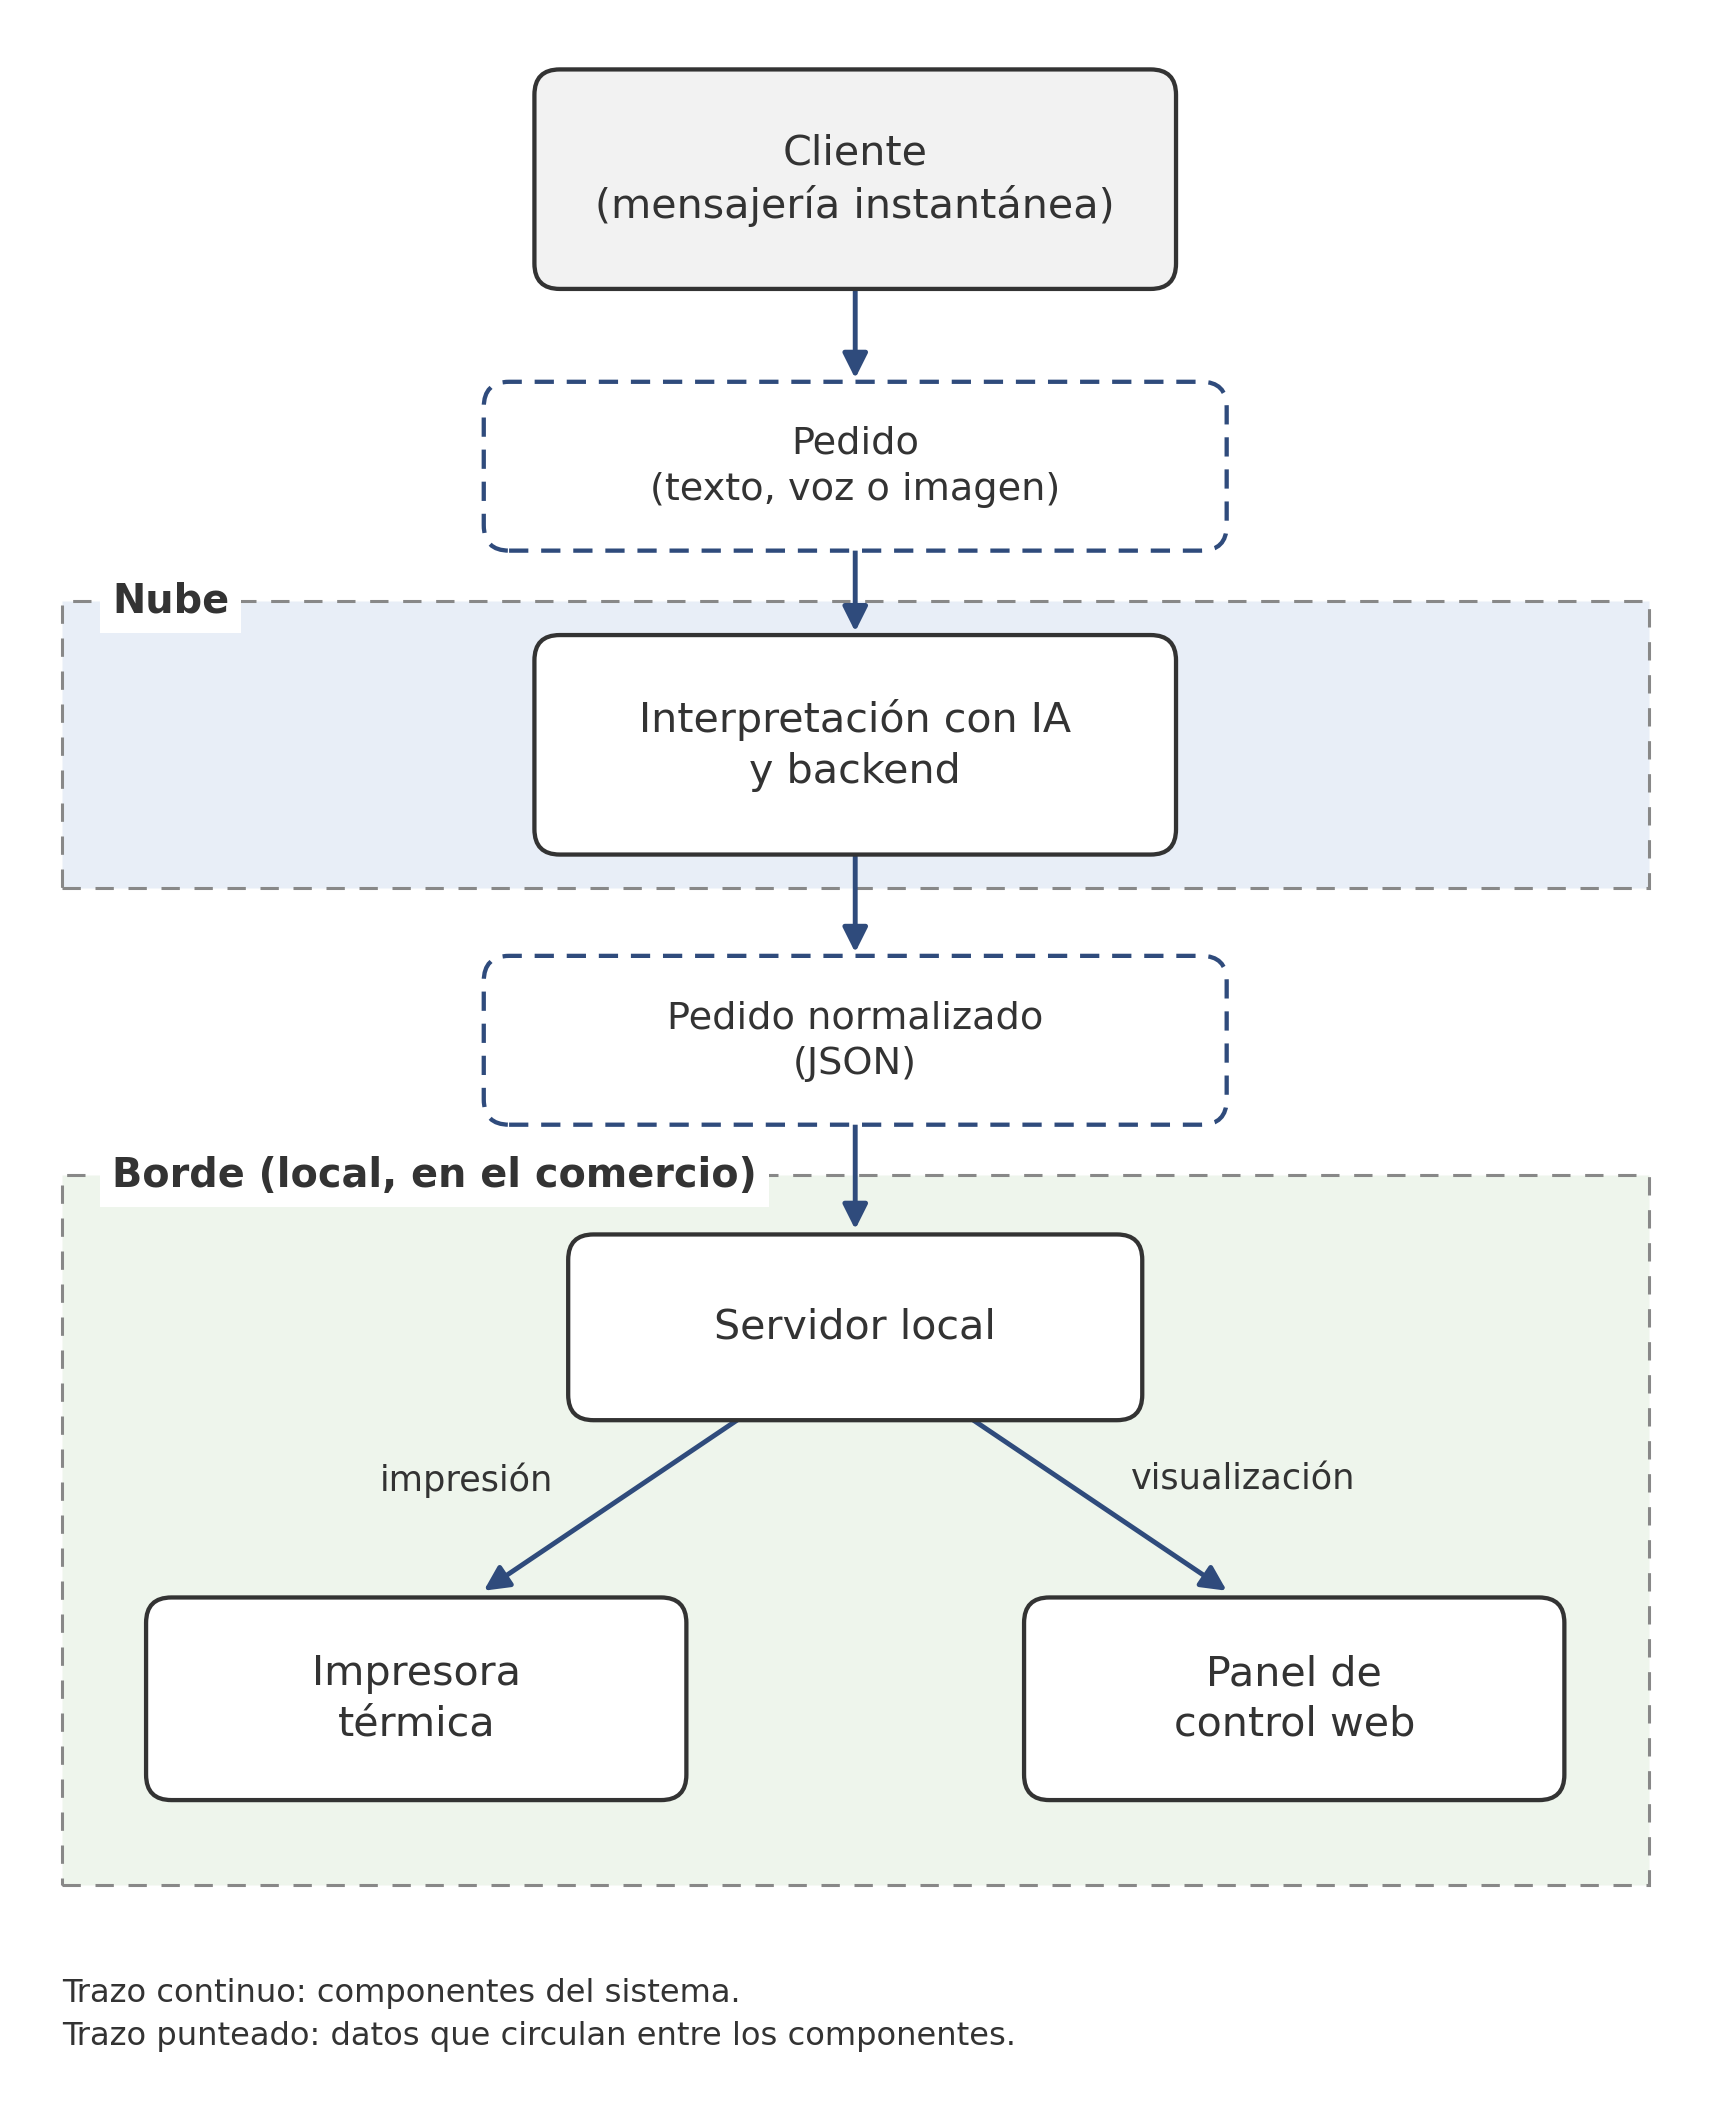
\includegraphics[width=0.9\textwidth]{Figures/diagrama_conceptual.png}
	\caption{Esquema conceptual del sistema: capas, componentes y flujo de datos.}
	\label{fig:diagrama_conceptual}
\end{figure}
 
%----------------------------------------------------------------------------------------
%	SECTION 2
%----------------------------------------------------------------------------------------
 
\section{Contexto y motivación}
\label{sec:contexto}
 
El trabajo se desarrolló para la Tienda de frutas Luján, un comercio minorista de frutas y verduras que recibe sus pedidos principalmente a través de mensajería instantánea. En la operación actual, un integrante del negocio lee cada mensaje entrante, interpreta su contenido (que puede llegar como texto, audio o imagen), normaliza los nombres y las cantidades de los productos y transcribe el pedido a un formato que permita su preparación y despacho.
 
Este proceso manual presenta varias limitaciones. En primer lugar, consume tiempo del personal que podría destinarse a la atención y a la preparación de los pedidos, y su capacidad se satura en los horarios de mayor demanda. En segundo lugar, la transcripción manual es propensa a errores de interpretación, especialmente ante mensajes de voz extensos, listas manuscritas poco legibles o denominaciones ambiguas de un mismo producto. En tercer lugar, al no existir un registro estructurado de los pedidos, se pierde trazabilidad: resulta difícil reconstruir el historial de un cliente, auditar un pedido puntual o extraer información agregada para la gestión comercial.
 
La motivación del desarrollo es, entonces, doble. Por un lado, se busca reducir los tiempos operativos y los errores humanos automatizando la recepción, la interpretación y la impresión de los pedidos. Por el otro, se procura hacerlo con una solución accesible y de bajo costo, adecuada a la realidad de un comercio que no dispone de infraestructura tecnológica avanzada ni de personal técnico especializado. Esta última condición es la que justifica el enfoque de computación de borde: procesar y actuar localmente permite que la operación crítica (la impresión del ticket para armar el pedido) siga funcionando con baja latencia y sin depender por completo de la disponibilidad de servicios remotos.
 
%----------------------------------------------------------------------------------------
%	SECTION 3
%----------------------------------------------------------------------------------------
 
\section{Estado del arte}
\label{sec:estado_arte}
 
La automatización de la recepción de pedidos en el comercio minorista puede abordarse desde distintos paradigmas, que se diferencian principalmente por dónde se ejecuta el procesamiento y por el grado de adaptación al canal de mensajería informal. A continuación, se revisan las alternativas existentes y se las contrasta con el enfoque adoptado en este trabajo.
 
\subsection{Soluciones basadas en la nube}
\label{subsec:soluciones_nube}
 
Una parte importante de las soluciones comerciales de gestión de pedidos y punto de venta se ofrece bajo el modelo de software como servicio, con todo el procesamiento centralizado en la nube. Entre las plataformas más conocidas se encuentran Shopify \cite{shopifypos} y, en el mercado local, Tiendanube \cite{tiendanubepdv}, que ofrecen soluciones de punto de venta y gestión de pedidos. Estas plataformas ofrecen paneles de administración, reportes y, en algunos casos, integración con canales de mensajería. Su principal ventaja es que no requieren infraestructura local más allá de un dispositivo con conexión a Internet. Sus limitaciones, en el contexto de este trabajo, son la dependencia total de la conectividad para operar, los costos recurrentes de suscripción y la escasa capacidad de personalización frente a un flujo de pedidos informal y no estructurado como el que se recibe por mensajería.
 
\subsection{Plataformas de automatización de mensajería}
\label{subsec:plataformas_mensajeria}
 
Existen plataformas y herramientas de automatización de flujos de trabajo que permiten conectar canales de mensajería con otros servicios mediante reglas o disparadores, como n8n \cite{n8n} o Zapier \cite{zapier}. Estas soluciones habilitan respuestas automáticas y la orquestación de tareas, pero por sí solas no resuelven la interpretación semántica de un pedido expresado en lenguaje natural, en audio o en una imagen. Para ello deben combinarse con modelos de procesamiento de lenguaje, reconocimiento de voz y reconocimiento óptico de caracteres (OCR, del inglés \textit{Optical Character Recognition}).
 
\subsection{Enfoques de borde e híbridos}
\label{subsec:enfoques_borde}
 
Frente a los esquemas puramente centralizados, la computación de borde propone ejecutar parte del procesamiento cerca del origen de los datos \cite{shi2016edge, satyanarayanan2017emergence}. En el comercio minorista, este enfoque resulta atractivo cuando existe una actuación física local, como la impresión de un ticket, que debe ocurrir con baja latencia y tolerancia a fallos de conectividad. Las arquitecturas híbridas, que combinan un nodo local con servicios en la nube, permiten equilibrar la capacidad de cómputo de la nube con la inmediatez y la resiliencia del procesamiento local \cite{tong2016hierarchical}.
 
\subsection{Comparación y posicionamiento del trabajo}
\label{subsec:comparacion_arte}
 
En la tabla \ref{tab:comparacion_arte} se comparan los tres paradigmas descriptos según los criterios más relevantes para el caso de uso abordado. El trabajo desarrollado se posiciona en el enfoque híbrido: delega en la nube las tareas de mayor demanda de cómputo (la interpretación de los mensajes mediante modelos de IA) y ejecuta en el borde la actuación crítica y de baja latencia (la impresión local del pedido), con lo que se busca un compromiso entre costo, personalización y disponibilidad adecuado a un comercio de baja complejidad tecnológica.
 
\begin{table}[h]
\centering
\caption{Comparación de paradigmas para la automatización de pedidos en el comercio minorista.}
\label{tab:comparacion_arte}
\begin{tabular}{p{3.2cm} p{2.6cm} p{2.6cm} p{2.6cm}}
\hline
Criterio & Nube pura & Automatización de mensajería & Enfoque híbrido (este trabajo) \\
\hline
Procesamiento local & No & Parcial & Sí (actuación local) \\
Dependencia de conectividad & Alta & Alta & Media \\
Personalización del flujo & Baja & Media & Alta \\
Costo de infraestructura & Bajo & Bajo & Bajo/Medio \\
Trazabilidad estructurada & Variable & Baja & Alta \\
\hline
\end{tabular}
\end{table}
 
%----------------------------------------------------------------------------------------
%	SECTION 4
%----------------------------------------------------------------------------------------
 
\section{Objetivos del trabajo}
\label{sec:objetivos}
 
El objetivo general del trabajo fue diseñar e implementar un sistema de automatización de pedidos. El sistema abarca la recepción, la interpretación y el procesamiento de los pedidos de un mercado de frutas y verduras recibidos a través de mensajería. De este modo se buscó reducir los tiempos operativos, minimizar los errores humanos y mejorar la trazabilidad de la operación comercial.
 
Para alcanzarlo, se definieron los siguientes objetivos específicos, formulados de manera concreta y verificable:
 
\begin{itemize}
	\item Capturar de forma automática los pedidos entrantes por el canal de mensajería, en sus distintos formatos: texto, voz e imagen.
	\item Interpretar el contenido de cada pedido mediante modelos de inteligencia artificial, identificando productos, cantidades y unidades, y normalizando denominaciones equivalentes de un mismo producto.
	\item Generar, a partir de esa interpretación, un pedido en formato estructurado y persistirlo de manera que quede registrada la trazabilidad completa, desde la recepción hasta la impresión.
	\item Imprimir automáticamente el pedido en una impresora térmica conectada a un servidor local, garantizando la actuación en el borde con baja latencia.
	\item Establecer una comunicación segura entre el servidor local y los servicios en la nube.
	\item Proveer un panel web que permita visualizar los pedidos en tiempo real, el historial y métricas básicas de operación.
	\item Validar el sistema en condiciones reales de operación en el comercio.
\end{itemize}
 
El alcance del trabajo se limita al flujo de recepción, interpretación, impresión y visualización de pedidos. Las tecnologías y componentes de terceros empleados en la construcción del sistema se describen en el capítulo \ref{Chapter2}, mientras que el diseño y la implementación de la arquitectura se detallan en el capítulo \ref{Chapter3}.
 